\documentclass{article}
\usepackage{tikz}
\usepackage{amsmath}
\usepackage{paralist}
\title{CMPS 130: HW 1 \\ {\small \copyright C. Seshadhri, 2019} \\ {\small Completed by Sankalp Chaubey} \\ {\small 2/5/2019} \\ {\small CruzID: schaubey} }
\date{}

\begin{document}
\maketitle

\medskip

\begin{compactenum}
\item (1.5 points) An \emph{all-NFA} $M$ is a 5-tuple $(Q,\Sigma,\delta,q_0,F)$
that accepts a string $x$ if \emph{every possible state} that $M$ could be in after
reading $x$ is an accepting state. (This is different from a standard NFA, where
only one possible non-deterministic path needs to lead to an accepting state.)
Prove that all-NFAs recognize the class of regular languages. \medskip

\textbf{Basis: } Suppose there is a regular language A. There must exist a  \emph { DFA B} that accepts this language A. 
This can be shown by \emph { L(D)=A. } We can use this\emph{ DFA B} to emulate an All-NFA, 
due to the fact that \emph {DFA B} accepts any string that is a part of lanuage A. \medskip

\textbf{Proof: } Suppose A is a language such that there is an \emph{all-NFA N} such that \emph{L(N)=A}.
The next step to prove this is to construct an NFA or DFA that recognizes this language. 
If we utilize the All-NFA defined earlier as a regular NFA, there will be strings that are not part of the language A that would
reach acceptance state as well. 
To address this, create an  and a \emph{all-NFA} $M$ is a 5-tuple $(Q,\Sigma,\delta,q_0,F)$ and a  \emph{DFA} $C$ is a 5-tuple $(Q',\Sigma,\delta',q'_0,F')$
Note that the accept state is  \emph{F'=P(F)}. When the simulated NFA ends all of the branches in accept states, the DFA will also reach acceptance. 
This will prove that All-NFAs recognize the class of regular languages.

\medskip
\item (1.5 points) Let $L$ be a regular language. Define $\textrm{PREFIX}(L) = \{x | \exists w, xw \in L\}$.
(Thus, $\textrm{PREFIX}(L)$ contains all prefixes of strings in $L$.) Prove that
$\textrm{PREFIX}(L)$ is regular.\medskip

\textbf{Basis: } Let \emph{L=L(M)} where DFA $M$ is a 5-tuple $(Q,\Sigma,\delta,q_0,F)$. Assume all states
are reachable from the start state of Q.  \medskip

\textbf{Proof: } Create a second \emph{DFA} $B$ which is defined by a  5-tuple $(Q,\Sigma,\delta,q_0,F')$. 
Using \emph {DFA} $B$, we can show \emph {Prefix(L)} is regular.  The difference between the definition of \emph{ DFA} $M$ and $B$, 
is that \emph{DFA} $B$ has a different acceptance state, denoted by F'.  \medskip

If and only if these conditions are met, \emph {Prefix(L)} will be regular: \medskip 
\begin{enumerate}
    \item If $\delta$(s,x)=q, then in  $\textrm{PREFIX}(L) = \{x \in L\}$ since  $\delta$(s,xw)=  ${F \in L} $.
    \item  Iff there is a path from \emph{q} to the accepting state of \emph{f} of the original \emph{DFA} $M$, 
	\emph{q} will reach the acceptance state\emph{ F'} of \emph{DFA} $B$. 
\end{enumerate}
\emph {Prefix(L)} is regular iff both the above conditions are met.



\medskip
\item (1.5 points) Define a pebbling finite state automaton (PFSA) as follows. Start with a
DFA $M$, and an arbitrary number of pebbles at the start state. Consider input $x$. Every time
$M$ processes a symbol of $x$, it \emph{non-deterministically} chooses to move
one of the pebbles, according to the transition function of $M$. At the end, if an accepting
state contains a pebble, then $x$ is accepted. More generally, $x$ is accepted
by $M$ if there exists a number of starting pebbles, and a sequence of moves that 
leads to some pebble ending at an accepting state. Prove that the set of languages
recognized by PFSAs is exactly the set of regular languages. \medskip

\textbf{Basis: } Due to the fact that a pebble in a PFSA can be moved at a stage of processing input, and there can be an arbitrary amount of pebbles, this machine would allow the user
to process any symbol as granted they are not limited on pebbles. Due to this design, it is not a matter of whether PFSA accepts regular or non-regular languages. Simply,
the set of regular languages will allow the second \emph{DFA} to reach an acceptance state. \medskip

\textbf {Proof: } Since the \emph {PFSA} is based upon a \emph {DFA}, we may construct both of each. If the language accepted by a the \emph {PFSA} is able to reach acceptance state, it will also cause the \emph {DFA} to reach the acceptance state.
These will be defined as such a \emph{PFSA} $M$ is a 5-tuple $(Q,\Sigma,\delta,q_0,F)$ with a pebble value, and a  \emph{DFA} $C$ is a 5-tuple $(Q',\Sigma,\delta',q'_0,F')$.
Let the language of the DFA be a regular language, and let the language of the PFSA be specific to the PFSA for the purpose of this proof. 
Note that the accept state is  \emph{F'=P(F)}. When the simulated PFSA in an acceptance state, the DFA will also reach acceptance. If the string is not recognized by the \emph{DFA} then it will not reach an acceptance state, thus whether or not
the PFSA accepts the same class of regular languages. 
\medskip
\item (1.5 points) Prove that these are not regular languages. (Let the alphabet $\Sigma = \{0,1\}$.)
\begin{enumerate}
    \item The set of strings that are \emph{not} of the form $ww$. (Meaning, the strings
    that are not formed by a double repetition of another string.)
    \item  $C = \{1^ky \ | \ y \textrm{ has at most $k$ 1s}, k \geq 1\}$.
\end{enumerate}
 \medskip
\textbf{Proof of Part A:} If \emph{A} is a regular language \emph{A} , then \emph{A}  has a "pumping length" of \emph{p} such that any string \emph{s} where $\mid s \mid$$\leq$ $p$,
may be divided into 3 parts, S=XYZ such that the pumping lemma cases hold. Let \emph{w=ww=($0^{p}$$1^{p}$$0^{p}$$1^{p}$)}. 
Using the pumping lemma,  $\mid xy \mid$$\leq$ $p$ and  $\mid y \mid$$\geq$ $1$, and p=7. Utilizing this pumping length, there will be more 0s in the x portion of the string in \emph { x$y^{i}$z}. 
This causes any string of the form ww to fail Case 1 of the pumping lemma since w$\neq$w $\in ww\ $. Due to this, any string of the form ww is not regular. 
The question asks strings that are not of the form ww. Due to the fact that the language fromed by the set of strings of the form \emph{ww} is not regular, a language not of this form may or not be regular.
Since A is non-regular, if its complement $\bar{A}$ were regular, $\overline{\overline{A}}$ then must be regular as well by the complementation lemma of regular languages.
\medskip

\textbf{Proof of Part B:} Assume that \emph{C} is regular, if \emph{C} is a regular language \emph{C} , then \emph{C}  has a "pumping length" of \emph{p} such that any string \emph{s} where $\mid s \mid$ $\leq$ $p$,
may be divided into 3 parts, S=xyz such that the pumping lemma cases hold. Using the string S of\emph{ $1^{p}$$0^{p}$$1^{p}$}. By the pumping lemma, it is required that s must be split into 3 pieces;
where s=abz, while ab $\leq$1. Using, b= $1^{i}$ for some i$\geq$1. \medskip
By pumping lemma we can re-write our string: \emph{ac}= \emph{ $1^{p-i}$$0^{p}$$1^{p}$}.
We can see that ac satisfies the parameters required by the pumping lemma as stated above, this contradicts the assumption that C is regular. 
Thus proving C as non-regular. Since C is non-regular, if its complement $\bar{C}$ were regular, $\overline{\overline{C}}$ then must be regular as well by the complementation lemma of regular languages.

\medskip
\item (1 point) (Let $\Sigma = \{0,1\}$.) Curiously, $B = \{1^ky \ | \ y \textrm{ has at least $k$ 1s}, k \geq 1\}$ is regular.
Prove that.

\medskip
\textbf{Proof:}
 Due the fact that the string in \emph{Language} $A$ must start with a 1, it must also contain another 1 in the y-segment. 
Any string that contains more than a singular '1' matches the requirement given by the definition of k=1. The string must also start with 1, and have another 1 as part of the string in order to balance and satisfy the pumping lemma.
Using A which can be dscribed by 1 o 0* o 1 o ($0 \cup 1$), this is a regular expression that is a part of \emph{L(B)}. 
We may also use a DFA to prove this.  Create a  \emph{DFA} $C$ as a 5-tuple $(Q,\Sigma,\delta,q_0,F)$. Allow this DFA to have states where the path to acceptance is $(q_0, q_1, q_2)$, with $q_2$ being the acceptance state, and q3 being a failure state. If entering the string 1 o 0* o 1 o ($0 \cup 1$) into this DFA, it will pass it to acceptance if the sequence follows the form of this regular expression. This proves that A is a regular language.
\medskip
\item (1.5 points)  The rotational closure of a language $L$ is defined $\textrm{RC}(L) = \{xy | yx \in L\}$.
Prove that regular languages are closed under rotational closures.
\medskip

\textbf{Basis:} If \emph{L} is a regular language, then it is accepted by a Finite Automata. We can create two DFAs, one for the string xy, and one to process yx. The second DFA can be made by simply switching the initial and final states, and reversing the directions of the transitions. If both DFAS reach an acceptance state then the languages are closed by reversal. 

\medskip
\textbf{Proof:}
\begin{center}
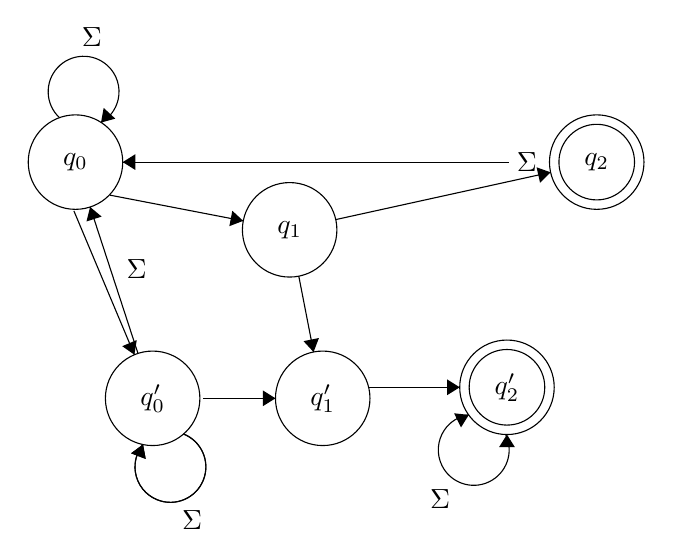
\begin{tikzpicture}[scale=0.2]
\tikzstyle{every node}+=[inner sep=0pt]
\draw [black] (24.2,-22.5) circle (3);
\draw (24.2,-22.5) node {$q_0$};
\draw [black] (37.8,-26.8) circle (3);
\draw (37.8,-26.8) node {$q_1$};
\draw [black] (57.3,-22.5) circle (3);
\draw (57.3,-22.5) node {$q_2$};
\draw [black] (57.3,-22.5) circle (2.4);
\draw [black] (29.1,-37.5) circle (3);
\draw (29.1,-37.5) node {$q'_0$};
\draw [black] (39.9,-37.5) circle (3);
\draw (39.9,-37.5) node {$q'_1$};
\draw [black] (51.6,-36.8) circle (3);
\draw (51.6,-36.8) node {$q'_2$};
\draw [black] (51.6,-36.8) circle (2.4);
\draw [black] (51.7,-22.5) -- (27.2,-22.5);
\draw (52.2,-22.5) node [right] {$\Sigma$};
\fill [black] (27.2,-22.5) -- (28,-23) -- (28,-22);
\draw [black] (23.193,-19.686) arc (227.41806:-60.58194:2.25);
\draw (25.24,-15.2) node [above] {$\Sigma$};
\fill [black] (25.82,-19.99) -- (26.73,-19.74) -- (25.99,-19.06);
\draw [black] (26.4,-24.6) -- (34.85,-26.23);
\fill [black] (34.85,-26.23) -- (34.16,-25.59) -- (33.97,-26.57);
\draw [black] (40.73,-26.15) -- (54.37,-23.15);
\fill [black] (54.37,-23.15) -- (53.48,-22.83) -- (53.7,-23.81);
\draw [black] (24.1,-25.6) -- (27.94,-34.73);
\fill [black] (27.94,-34.73) -- (28.09,-33.8) -- (27.17,-34.19);
\draw [black] (38.38,-29.74) -- (39.32,-34.56);
\fill [black] (39.32,-34.56) -- (39.66,-33.67) -- (38.68,-33.87);
\draw [black] (42.8,-36.8) -- (48.6,-36.8);
\fill [black] (48.6,-36.8) -- (47.8,-36.3) -- (47.8,-37.3);
\draw [black] (31.053,-39.762) arc (68.53446:-219.46554:2.25);
\draw (31.6,-44.61) node [below] {$\Sigma$};
\fill [black] (28.49,-40.43) -- (27.73,-40.99) -- (28.66,-41.35);
\draw [black] (31.053,-39.762) arc (68.53446:-219.46554:2.25);
\fill [black] (28.49,-40.43) -- (27.73,-40.99) -- (28.66,-41.35);
\draw [black] (32.3,-37.5) -- (36.9,-37.5);
\fill [black] (36.9,-37.5) -- (36.1,-37) -- (36.1,-38);
\draw [black] (51.6,-39.8) -- (51.6,-39.8);
\fill [black] (51.6,-39.8) -- (51.1,-40.6) -- (52.1,-40.6);
\draw [black] (28.17,-34.65) -- (25.13,-25.35);
\fill [black] (25.13,-25.35) -- (24.9,-26.27) -- (25.86,-25.96);
\draw (27.42,-29.32) node [right] {$\Sigma$};
\draw [black] (51.511,-39.787) arc (26.0304:-261.9696:2.25);
\draw (47.36,-43.26) node [below] {$\Sigma$};
\fill [black] (49.18,-38.55) -- (48.24,-38.45) -- (48.68,-39.35);
\end{tikzpicture}
\end{center}
Let \emph{DFA} $M$ be a 5-tuple $(Q,\Sigma,\delta,q_0,F)$ and a  \emph{DFA} $C$ be a 5-tuple $(Q',\Sigma,\delta',q'_0,F')$. 
Assume that the \emph {DFA} with states denoted by an apostrophe is \emph{C}. \emph{C} contains the states of same states and steps as \emph{M} simply with the finish state and acceptance state swapped.   Let the \emph {DFA M} have accept a language with a string xy, and let \emph {DFA C} accept a language with string yx. 
The \emph{DFAS} above demonstrate how these two \emph {DFAS} could work in conjuction to establish closure by reversal and rotational closure. 
\medskip
\item (1.5 points) Let $L$ and $M$ be languages.
Define language $L \ominus M = \{x | x \in L \ \textrm{and $x$ does not contain any string of $M$ as substring}\}$.
Prove that: if $L$ and $M$ are regular, $L \ominus M$ is regular.

\medskip
\textbf{Proof:}
The symmetric difference of L and M can be described as: L$\Delta$M= (L/ M) $\cup$ (M/ L). If both L and M are both part of the alphabet $(\sigma)$, both are regular languages, then the symetric difference given by L$\Delta$M.
If both L and M are regular then their complements  $\bar{L}$ and  $\bar{M}$ are also both regular. This implies the instersections of L $(\cap)$ $\bar{M}$ and M $(\cap)$ $\bar{L}$ are also regular, and therefore the union ( L $(\cap)$  $\bar{M}$) and 
( M$(\cap)$  $\bar{L}$) is also regular.  This gives: ( L $(\cap)$  $\bar{M}$)$(\cup)$( M$(\cap)$  $\bar{L}$)= L$\Delta$M. This is possible due to regular
languages being closed under union, intersection, and complementation. L and M were regular through each of these steps. Thus proving that the ominus operation in between L and M are regular.
\end{compactenum}



\end{document}
